\documentclass[]{article}
\usepackage{lmodern}
\usepackage[compact]{titlesec}
\usepackage{amssymb,amsmath}
\usepackage{ifxetex,ifluatex}
\usepackage{fixltx2e} % provides \textsubscript
\ifnum 0\ifxetex 1\fi\ifluatex 1\fi=0 % if pdftex
  \usepackage[T1]{fontenc}
  \usepackage[utf8]{inputenc}
\else % if luatex or xelatex
  \ifxetex
    \usepackage{mathspec}
  \else
    \usepackage{fontspec}
  \fi
  \defaultfontfeatures{Ligatures=TeX,Scale=MatchLowercase}
\fi
% use upquote if available, for straight quotes in verbatim environments
\IfFileExists{upquote.sty}{\usepackage{upquote}}{}
% use microtype if available
\IfFileExists{microtype.sty}{%
\usepackage{microtype}
\UseMicrotypeSet[protrusion]{basicmath} % disable protrusion for tt fonts
}{}
\usepackage[margin=1in]{geometry}
\usepackage{hyperref}
\hypersetup{unicode=true,
            pdftitle={Final Course Project},
            pdfauthor={Darryl Buswell},
            pdfborder={0 0 0},
            breaklinks=true}
\urlstyle{same}  % don't use monospace font for urls
\usepackage{longtable,booktabs}
\usepackage{graphicx,grffile}
\makeatletter
\def\maxwidth{\ifdim\Gin@nat@width>\linewidth\linewidth\else\Gin@nat@width\fi}
\def\maxheight{\ifdim\Gin@nat@height>\textheight\textheight\else\Gin@nat@height\fi}
\makeatother
% Scale images if necessary, so that they will not overflow the page
% margins by default, and it is still possible to overwrite the defaults
% using explicit options in \includegraphics[width, height, ...]{}
\setkeys{Gin}{width=\maxwidth,height=\maxheight,keepaspectratio}
\IfFileExists{parskip.sty}{%
\usepackage{parskip}
}{% else
\setlength{\parindent}{0pt}
\setlength{\parskip}{6pt plus 2pt minus 1pt}
}
\setlength{\emergencystretch}{3em}  % prevent overfull lines
\providecommand{\tightlist}{%
  \setlength{\itemsep}{0pt}\setlength{\parskip}{0pt}}
\setcounter{secnumdepth}{0}
% Redefines (sub)paragraphs to behave more like sections
\ifx\paragraph\undefined\else
\let\oldparagraph\paragraph
\renewcommand{\paragraph}[1]{\oldparagraph{#1}\mbox{}}
\fi
\ifx\subparagraph\undefined\else
\let\oldsubparagraph\subparagraph
\renewcommand{\subparagraph}[1]{\oldsubparagraph{#1}\mbox{}}
\fi

%%% Use protect on footnotes to avoid problems with footnotes in titles
\let\rmarkdownfootnote\footnote%
\def\footnote{\protect\rmarkdownfootnote}

%%% Change title format to be more compact
\usepackage{titling}

% Create subtitle command for use in maketitle
\newcommand{\subtitle}[1]{
  \posttitle{
    \begin{center}\large#1\end{center}
    }
}

\setlength{\droptitle}{-2em}
  \title{Final Course Project}
  \pretitle{\vspace{\droptitle}\centering\huge}
  \posttitle{\par}
\subtitle{MSPA PREDICT 422-DL-56 LEC}
  \author{Darryl Buswell}
  \preauthor{\centering\large\emph}
  \postauthor{\par}
  \date{}
  \predate{}\postdate{}

\begin{document}
\maketitle

\section{1 Introduction}\label{introduction}

This document presents the results of the final assessment for the
Masters of Science in Predictive Analytics course: PREDICT 422. This
assessment required the student to develop a predictive model in order
to identify donors that are likely to respond to a mailing campaign, and
once identified, estimate the net donation amount that may result from
targeting those donors as part of a new mailing campaign.

For this assessment, we leverage a dataset which contains variables
relating to previous donors. We use this data to first assess which
variables have the greatest `importance' in determining both the chance
of response to a mailing campaign as well as the likely donation amount.
We then use this reduced dataset to fit six classification models to
predict chance of donation, and six regression models to predict likely
donation amount. Optimal models are selected and subsequently used in
order to estimate the expected net revenue from conducting a new
targeted mailing campaign, accounting for the cost of mailing each
donor.

\section{2 Data}\label{data}

The dataset includes 8,009 records and 20 features of donor data. The
features capture results from previous donation campaigns and properties
of each donor. Features are broken up into 19 integer and one long
variable type. A description of each feature can be found in the table
below.

\subsubsection{Table 2.1 Feature
Descriptions}\label{table-2.1-feature-descriptions}

\begin{longtable}[]{@{}ll@{}}
\toprule
\begin{minipage}[b]{0.20\columnwidth}\raggedright\strut
Feature\strut
\end{minipage} & \begin{minipage}[b]{0.74\columnwidth}\raggedright\strut
Description\strut
\end{minipage}\tabularnewline
\midrule
\endhead
\begin{minipage}[t]{0.20\columnwidth}\raggedright\strut
REG1 REG2 REG3 REG4\strut
\end{minipage} & \begin{minipage}[t]{0.74\columnwidth}\raggedright\strut
Region which the donor belongs to (1 = belongs to region 0 = does not
belong)\strut
\end{minipage}\tabularnewline
\begin{minipage}[t]{0.20\columnwidth}\raggedright\strut
HOME\strut
\end{minipage} & \begin{minipage}[t]{0.74\columnwidth}\raggedright\strut
(1 = homeowner 0 = not a homeowner)\strut
\end{minipage}\tabularnewline
\begin{minipage}[t]{0.20\columnwidth}\raggedright\strut
CHLD\strut
\end{minipage} & \begin{minipage}[t]{0.74\columnwidth}\raggedright\strut
Number of children\strut
\end{minipage}\tabularnewline
\begin{minipage}[t]{0.20\columnwidth}\raggedright\strut
HINC\strut
\end{minipage} & \begin{minipage}[t]{0.74\columnwidth}\raggedright\strut
Household income (7 categories)\strut
\end{minipage}\tabularnewline
\begin{minipage}[t]{0.20\columnwidth}\raggedright\strut
GENF\strut
\end{minipage} & \begin{minipage}[t]{0.74\columnwidth}\raggedright\strut
Gender (0 = Male 1 = Female)\strut
\end{minipage}\tabularnewline
\begin{minipage}[t]{0.20\columnwidth}\raggedright\strut
WRAT\strut
\end{minipage} & \begin{minipage}[t]{0.74\columnwidth}\raggedright\strut
Wealth Rating (0-9 with 0 being lowest wealth)\strut
\end{minipage}\tabularnewline
\begin{minipage}[t]{0.20\columnwidth}\raggedright\strut
AVHV\strut
\end{minipage} & \begin{minipage}[t]{0.74\columnwidth}\raggedright\strut
Average Home Value in potential donor's neighborhood in \$
thousands\strut
\end{minipage}\tabularnewline
\begin{minipage}[t]{0.20\columnwidth}\raggedright\strut
INCM\strut
\end{minipage} & \begin{minipage}[t]{0.74\columnwidth}\raggedright\strut
Median Family Income in potential donor's neighborhood in \$
thousands\strut
\end{minipage}\tabularnewline
\begin{minipage}[t]{0.20\columnwidth}\raggedright\strut
INCA\strut
\end{minipage} & \begin{minipage}[t]{0.74\columnwidth}\raggedright\strut
Average Family Income in potential donor's neighborhood in \$
thousands\strut
\end{minipage}\tabularnewline
\begin{minipage}[t]{0.20\columnwidth}\raggedright\strut
PLOW\strut
\end{minipage} & \begin{minipage}[t]{0.74\columnwidth}\raggedright\strut
Percent categorized as ``low income'' in potential donor's
neighborhood\strut
\end{minipage}\tabularnewline
\begin{minipage}[t]{0.20\columnwidth}\raggedright\strut
NPRO\strut
\end{minipage} & \begin{minipage}[t]{0.74\columnwidth}\raggedright\strut
Lifetime number of promotions received to date\strut
\end{minipage}\tabularnewline
\begin{minipage}[t]{0.20\columnwidth}\raggedright\strut
TGIF\strut
\end{minipage} & \begin{minipage}[t]{0.74\columnwidth}\raggedright\strut
Dollar amount of lifetime gifts to date\strut
\end{minipage}\tabularnewline
\begin{minipage}[t]{0.20\columnwidth}\raggedright\strut
LGIF\strut
\end{minipage} & \begin{minipage}[t]{0.74\columnwidth}\raggedright\strut
Dollar amount of largest gift to date\strut
\end{minipage}\tabularnewline
\begin{minipage}[t]{0.20\columnwidth}\raggedright\strut
RGIF\strut
\end{minipage} & \begin{minipage}[t]{0.74\columnwidth}\raggedright\strut
Dollar amount of most recent gift\strut
\end{minipage}\tabularnewline
\begin{minipage}[t]{0.20\columnwidth}\raggedright\strut
TDON\strut
\end{minipage} & \begin{minipage}[t]{0.74\columnwidth}\raggedright\strut
Number of months since last donation\strut
\end{minipage}\tabularnewline
\begin{minipage}[t]{0.20\columnwidth}\raggedright\strut
TLAG\strut
\end{minipage} & \begin{minipage}[t]{0.74\columnwidth}\raggedright\strut
Number of months between first and second gift\strut
\end{minipage}\tabularnewline
\begin{minipage}[t]{0.20\columnwidth}\raggedright\strut
AGIF\strut
\end{minipage} & \begin{minipage}[t]{0.74\columnwidth}\raggedright\strut
Average dollar amount of gifts to date\strut
\end{minipage}\tabularnewline
\bottomrule
\end{longtable}

Do note that the dataset was already separated into a training (3,984),
validation (2,018) and test (2,007) subset, according to the flag,
`PART'.

From an initial look at the data, we noted that the compiled R data
frame fails to distinguish between numeric and factor variables. As
such, prior to performing any data exploration, we converted all
variables with two or less levels to factor type and retained all other
variables as numeric type. This resulted in the identification of six
factor type variables, including, `REG1', `REG2', `REG3', `REG4', `HOME'
and `GENF'.

\section{3 Data Exploration}\label{data-exploration}

A number of exploration routines were conducted. These routines allowed
us to gain an understanding of potential data limitations, including
identifying variables which have missing observations, outlier
observations, or those variables which may benefit from transformation.

\subsection{3.1 Univariate Data
Analysis}\label{univariate-data-analysis}

As part of the univariate data analysis, summary statistics for all
numeric variables were calculated and observed. Summary statistics can
be found in the table below.

\subsubsection{Table 3.1.1 Numeric Variable Summary
Statistics}\label{table-3.1.1-numeric-variable-summary-statistics}

\begin{longtable}[]{@{}llllllll@{}}
\toprule
Feature & Mean & Median & s.d. & Min & Max & Miss & n\tabularnewline
\midrule
\endhead
chld & 1.7172 & 2 & 1.4017 & 0 & 5 & 0 & 8009\tabularnewline
hinc & 3.9086 & 4 & 1.4672 & 1 & 7 & 0 & 8009\tabularnewline
wrat & 6.9141 & 8 & 2.4286 & 0 & 9 & 0 & 8009\tabularnewline
avhv & 182.646 & 169 & 72.72 & 48 & 710 & 0 & 8009\tabularnewline
incm & 43.4742 & 38 & 24.7066 & 3 & 287 & 0 & 8009\tabularnewline
inca & 56.4281 & 51 & 24.8175 & 12 & 305 & 0 & 8009\tabularnewline
plow & 14.2332 & 10 & 13.4115 & 0 & 87 & 0 & 8009\tabularnewline
npro & 60.0312 & 58 & 30.3452 & 2 & 164 & 0 & 8009\tabularnewline
tgif & 113.0697 & 89 & 85.4751 & 23 & 2057 & 0 & 8009\tabularnewline
lgif & 22.9404 & 16 & 29.9479 & 3 & 681 & 0 & 8009\tabularnewline
rgif & 15.6618 & 12 & 12.4347 & 1 & 173 & 0 & 8009\tabularnewline
tdon & 18.8637 & 18 & 5.7832 & 5 & 40 & 0 & 8009\tabularnewline
tlag & 6.3632 & 5 & 3.7037 & 1 & 34 & 0 & 8009\tabularnewline
agif & 11.6807 & 10.23 & 6.5669 & 1.29 & 72.27 & 0 & 8009\tabularnewline
\bottomrule
\end{longtable}

We observed that the numeric variables do not suffer from missing
values. However, a few variables have a minimum value of zero,
suggesting zero-inflated data. We also noted that a comparison of the
min/max and standard deviation values of a number of variables suggests
the presence of outliers.

Histogram and box plots were also generated and reviewed for a large
subset of numeric variables, with the number of children (CHLD) and
amount of gifts to date (TGIF) selected for further discussion below.

\newpage

\paragraph{Figure 3.1.1 Histogram and Boxplot:
CHLD}\label{figure-3.1.1-histogram-and-boxplot-chld}

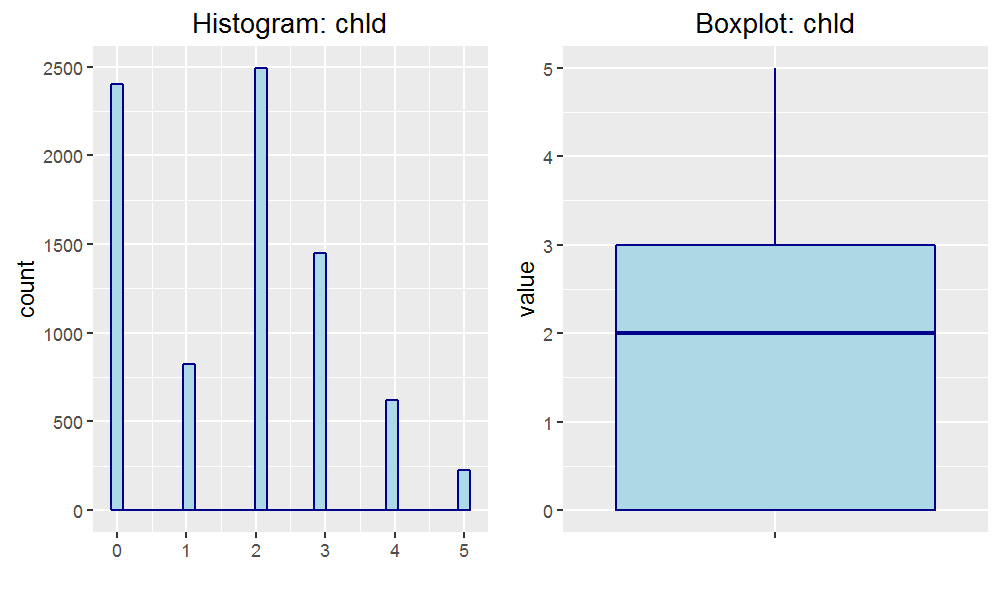
\includegraphics[height=3.33333in]{images/expl_num_chld.png}

\paragraph{Figure 3.1.2 Histogram and Boxplot:
TGIF}\label{figure-3.1.2-histogram-and-boxplot-tgif}

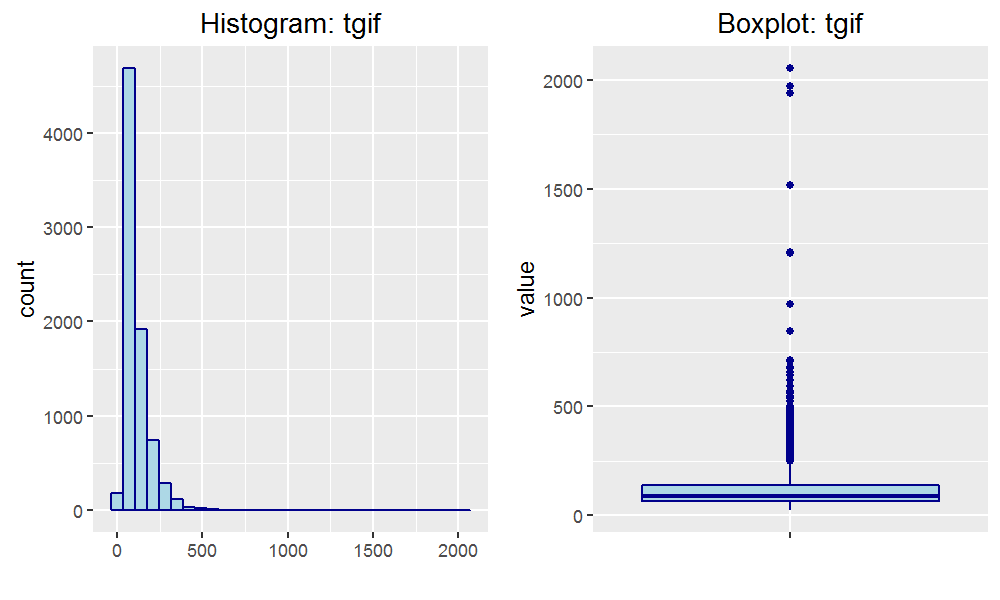
\includegraphics[height=3.33333in]{images/expl_num_tgif.png}

We immediately noticed that CHLD is zero-inflated, with many donors
reported as not having any children. We also noted that while TGIF is
more continuous in its nature than CHLD, this feature suffers from a
heavy positive skew. This is in-fact a common attribute of the majority
of features, with the greatest skew being noted for RGIF, INCA, INCM,
and PLOW. The result is a number of observations which could be classed
as outliers.

\subsection{3.2 Bivariate Data Analysis}\label{bivariate-data-analysis}

Since we intend on building a prediction model to determine both the
chance of response to a mailing campaign (DONR) and the likely donation
amount (DAMT), we have an interest in identifying variables which have
explanatory power over these two variables. As such, we calculated and
reviewed the Pearson correlation coefficient for all numeric variables
against our numeric response variable, DAMT. Correlations are shown in
the table below.

\subsubsection{Table 3.2.1 Correlation against
DAMT}\label{table-3.2.1-correlation-against-damt}

\begin{longtable}[]{@{}ll@{}}
\toprule
Feature & Correlation\tabularnewline
\midrule
\endhead
wrat & 0.231\tabularnewline
npro & 0.1458\tabularnewline
incm & 0.1453\tabularnewline
inca & 0.1294\tabularnewline
tgif & 0.1255\tabularnewline
avhv & 0.1112\tabularnewline
rgif & 0.0785\tabularnewline
agif & 0.0781\tabularnewline
lgif & 0.0768\tabularnewline
hinc & 0.0508\tabularnewline
tdon & -0.0922\tabularnewline
tlag & -0.1239\tabularnewline
plow & -0.1253\tabularnewline
chld & -0.5531\tabularnewline
\bottomrule
\end{longtable}

None of the variables have reported a strong correlation with DAMT, with
the greatest absolute correlation being reported by WRAT and CHLD.
However, the polarity of the majority of coefficients seems reasonable.
For example, a greater amount of wealth or having less children is
suggested to result in a greater donation amount.

Finally, we used bar plots to explore the relationship between the
categorical response variable (DONR) and each numeric variable. Two of
these plots have been selected for further discussion below.

\newpage

\paragraph{Figure 3.2.1 Boxplot: DONR vs.~NPRO /
PLOW}\label{figure-3.2.1-boxplot-donr-vs.npro-plow}

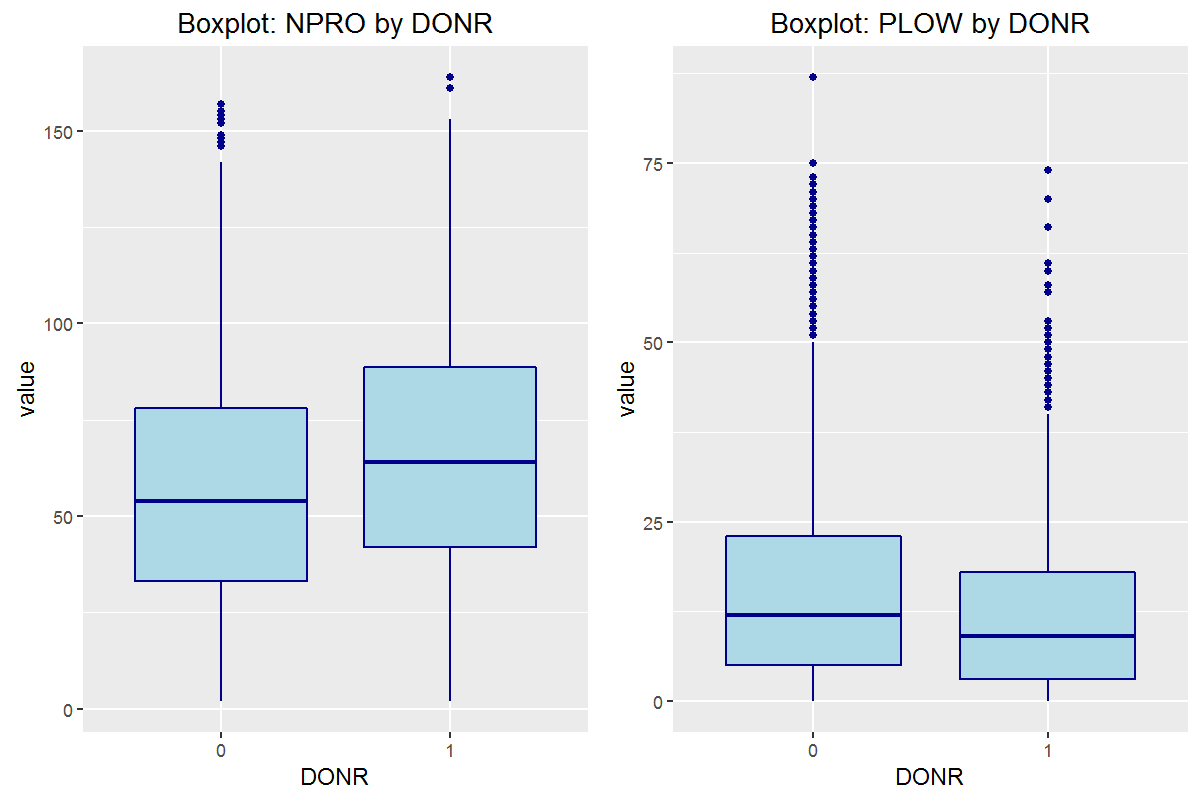
\includegraphics[height=3.33333in]{images/expl_boxcomp_1.png}

We can see that there are indeed recognizable differences in both the
mean and distribution for both features, depending on whether they are
associated with a positive or negative response to a mailing campaign.
For example, we see that those donors who did in-fact respond received a
greater number of promotions (NPRO) or had fewer people categorized as
`low income' within their neighborhood (PLOW).

\section{4 Data Pre-processing}\label{data-pre-processing}

As part of the data pre-processing routine, we looked towards dealing
with outlier observations for numeric variables. In many cases, the task
of identifying outlier observations can be a subjective practice. As
such, for this assessment, we took a statistical approach and targeted
those observations which fell outside the 1st and 99th percentile range.
Observations which met these criteria were replaced using the squish
function as part of the scales package in R, effectively resulting in a
newly created set of trimmed variables. Trimmed variables added to the
dataset and can be recognized by the suffix '\_T99'.

Next, we looked to transform the data by making a copy of each numeric
variable and performing a log transformation on each copy. Such a
transformation will help penalize extreme values and may aid in limiting
the identified heavy skew for a number of numeric distributions. All
transformed variables carry the suffix '\_LN'.

Finally, we looked towards creating dummies for each of the retained
factor variables. Dummy variables were named to include the prefix
`DUM\_', along with a suffix to represent the factor level. Note that
k-1 dummies were created, where k is the original number of levels for
each variable. This resulted in the creation of six dummies.

\section{5 Variable Importance}\label{variable-importance}

The data processing routine produced a data frame of 54 features, all of
numeric type. With such a large feature set, it was clear that any
subsequent model estimation would benefit from a further reduction in
variable count. To achieve this, we leveraged the varImp function as
part of the caret package in R to calculate the variable importance
according to both response variables. In both cases, variable importance
was calculated by fitting a Random Forest model, with `importance'
measured by the mean decrease in node impurity. Bar plots of the 20 most
important variables for both response variables are below.

\paragraph{Figure 5.1 Variable Importance:
DONR}\label{figure-5.1-variable-importance-donr}

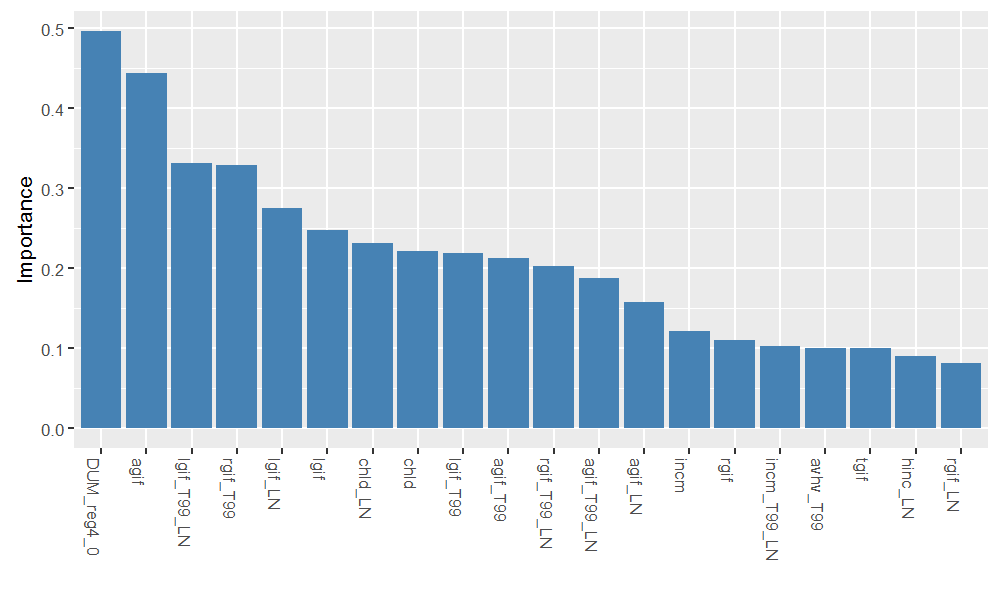
\includegraphics[height=3.02083in]{images/varimp_resp.png}

\paragraph{Figure 5.2 Variable Importance:
DAMT}\label{figure-5.2-variable-importance-damt}

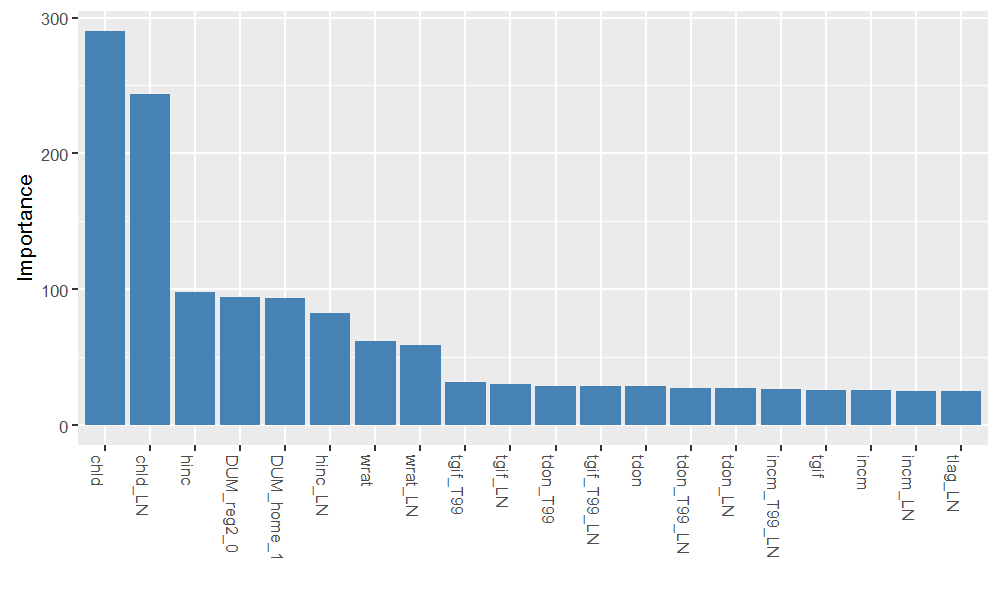
\includegraphics[height=3.02083in]{images/varimp_amt.png}

We can see some commonality between variable importance plots, with CHLD
and dummies for HOME and REG2 all within the top-10 rank for both
response variables. We also note a fairly quick drop-off in variable
importance beyond the first five variables within both plots. Based on
these results, we elected to pass the top-20 ranked variables by
importance through to our model estimation phase. We believe this
reduction provides a suitable trade-off both in terms of accuracy and
performance.

\section{6 Model Estimation}\label{model-estimation}

\subsection{6.1 Classification Modelling: Chance of
Response}\label{classification-modelling-chance-of-response}

For this assessment, we fit six classification based models in order to
predict the chance a donor will respond. These models include a Naive
Bayes, Random Forest, Lasso and Elastic-Net Regularized Generalized
Linear Model (GLMnet), Logit Boost, Linear Discriminant Analysis (LDA)
and k-Nearest Neighbors (kNN) classifier. In each case, we leverage the
train function as part of the caret package with a 3-fold
cross-validation sampling method, which was applied to the training data
and tested against the validation subset. Default parameters were used
for each model.

The in and out-of-sample Receiver Operating Characteristic (ROC) Curves
are shown for each model in Appendix A. From observing each ROC curve,
we note that both the Random Forest and kNN classifiers seem to have
overfit the training data since both returned an AUC greater than 0.99
over the training set yet returned a much lower AUC over the validation
set. The GLMnet and LDA classifiers seem to have delivered more
promising results however, returning an AUC of over 0.95 over both the
training and validation sets. Below we show the out-of-sample confusion
matrix for each model.

\paragraph{Table 6.1.1 Confusion Matrix: Classification Model
Comparison}\label{table-6.1.1-confusion-matrix-classification-model-comparison}

\begin{longtable}[]{@{}lllllllllll@{}}
\toprule
Naive Bayes & & & & Random Forest & & & & GLMnet & &\tabularnewline
& Pred: 0 & Pred: 1 & & & Pred: 0 & Pred: 1 & & & Pred: 0 & Pred:
1\tabularnewline
Actual: 0 & 811 & 163 & & Actual: 0 & 886 & 91 & & Actual: 0 & 895 &
94\tabularnewline
Actual: 1 & 208 & 836 & & Actual: 1 & 133 & 908 & & Actual: 1 & 124 &
905\tabularnewline
& & & & & & & & & &\tabularnewline
Logit Boost & & & & LDA & & & & kNN & &\tabularnewline
& Pred: 0 & Pred: 1 & & & Pred: 0 & Pred: 1 & & & Pred: 0 & Pred:
1\tabularnewline
Actual: 0 & 813 & 103 & & Actual: 0 & 873 & 81 & & Actual: 0 & 701 &
88\tabularnewline
Actual: 1 & 206 & 896 & & Actual: 1 & 146 & 918 & & Actual: 1 & 318 &
911\tabularnewline
\bottomrule
\end{longtable}

We can see that both the GLMnet and LDA classifiers have produced
similar true positive and true negative rates over the validation set.
That is, neither has a bias in performance towards classification of
positive or negative observations. Finally, we present a set of
performance metrics for each classifier in the table below.

\paragraph{Table 6.1.2 Performance Metrics: Classification Model
Comparison}\label{table-6.1.2-performance-metrics-classification-model-comparison}

\begin{longtable}[]{@{}lllllll@{}}
\toprule
Metric & Naive Bayes & Random Forest & GLMnet & Logit Boost & LDA &
kNN\tabularnewline
\midrule
\endhead
Accuracy & 0.8162 & 0.889 & 0.892 & 0.8469 & 0.8875 &
0.7988\tabularnewline
95\% CI LB & 0.7986 & 0.8745 & 0.8776 & 0.8304 & 0.8729 &
0.7806\tabularnewline
95\% CI UB & 0.8328 & 0.9024 & 0.9052 & 0.8623 & 9.01E-01 &
0.8161\tabularnewline
Kappa & 0.6324 & 0.7781 & 0.784 & 0.694 & 0.7751 & 0.5985\tabularnewline
Sensitivity & 0.8368 & 0.9089 & 0.9059 & 0.8969 & 0.9189 &
0.9119\tabularnewline
Specificity & 0.7959 & 0.8695 & 0.8783 & 0.7978 & 0.8567 &
0.6879\tabularnewline
Pos Pred Value & 0.8008 & 0.8722 & 0.8795 & 0.8131 & 0.8628 &
0.7413\tabularnewline
Neg Pred Value & 0.8326 & 0.9069 & 0.905 & 0.8876 & 0.9151 &
0.8885\tabularnewline
Prevalence & 0.495 & 0.495 & 0.495 & 0.495 & 0.495 &
0.495\tabularnewline
Detection Rate & 0.4143 & 0.45 & 0.4485 & 0.444 & 0.4549 &
0.4514\tabularnewline
Detection Prevalence & 0.5173 & 0.5159 & 0.5099 & 0.5461 & 0.5273 &
0.609\tabularnewline
Balanced Accuracy & 0.8164 & 0.8892 & 0.8921 & 0.8474 & 0.8878 &
0.7999\tabularnewline
\bottomrule
\end{longtable}

From a view of the performance metrics above, we can see that the GLMnet
model has demonstrated a superior AUC, accuracy and specificity compared
to the other models. As such, we have elected to use the GLMnet
classifier to predict the chance of response.

\subsection{6.2 Regression Modelling: Amount
Donated}\label{regression-modelling-amount-donated}

We next fit six regression based models in order to predict the amount
of donation. These models include a Multiple Linear Regression (MLR),
Random Forest, eXtreme Gradient Boost, Partial Least Squares, Ridge
Regression, and a Least Absolute Shrinkage and Selection Operator
(LASSO) estimator. Note that for the MLR, a stepwise variable selection
technique was used based on the Akaike Information Criterion (AIC). As
with the previous classification models, we employed a 3-fold
cross-validation sampling method, and maintained the same training and
validation split.

The in and out-of-sample actuals versus predictions for each model are
shown in Appendix A. We can see that each model seems to struggle with
outlier observations. We can extend the model assessment by observing
the model fit statistics for each in the below table. Note that negative
prediction values were taken as zero for the statistics shown in the
table below. That is, we interpret negative donation amounts to be zero.

\paragraph{Table 6.2.1 Performance Metrics: Regression Model
Comparison}\label{table-6.2.1-performance-metrics-regression-model-comparison}

\begin{longtable}[]{@{}lllllll@{}}
\toprule
\begin{minipage}[b]{0.11\columnwidth}\raggedright\strut
\strut
\end{minipage} & \begin{minipage}[b]{0.06\columnwidth}\raggedright\strut
MLR\strut
\end{minipage} & \begin{minipage}[b]{0.11\columnwidth}\raggedright\strut
Random Forest\strut
\end{minipage} & \begin{minipage}[b]{0.15\columnwidth}\raggedright\strut
eXtreme Grad Boost\strut
\end{minipage} & \begin{minipage}[b]{0.17\columnwidth}\raggedright\strut
Partial Least Squares\strut
\end{minipage} & \begin{minipage}[b]{0.14\columnwidth}\raggedright\strut
Ridge Regression\strut
\end{minipage} & \begin{minipage}[b]{0.06\columnwidth}\raggedright\strut
LASSO\strut
\end{minipage}\tabularnewline
\midrule
\endhead
\begin{minipage}[t]{0.11\columnwidth}\raggedright\strut
Training set\strut
\end{minipage} & \begin{minipage}[t]{0.06\columnwidth}\raggedright\strut
\strut
\end{minipage} & \begin{minipage}[t]{0.11\columnwidth}\raggedright\strut
\strut
\end{minipage} & \begin{minipage}[t]{0.15\columnwidth}\raggedright\strut
\strut
\end{minipage} & \begin{minipage}[t]{0.17\columnwidth}\raggedright\strut
\strut
\end{minipage} & \begin{minipage}[t]{0.14\columnwidth}\raggedright\strut
\strut
\end{minipage} & \begin{minipage}[t]{0.06\columnwidth}\raggedright\strut
\strut
\end{minipage}\tabularnewline
\begin{minipage}[t]{0.11\columnwidth}\raggedright\strut
MAE\strut
\end{minipage} & \begin{minipage}[t]{0.06\columnwidth}\raggedright\strut
0.8\strut
\end{minipage} & \begin{minipage}[t]{0.11\columnwidth}\raggedright\strut
0.36\strut
\end{minipage} & \begin{minipage}[t]{0.15\columnwidth}\raggedright\strut
0.25\strut
\end{minipage} & \begin{minipage}[t]{0.17\columnwidth}\raggedright\strut
1.25\strut
\end{minipage} & \begin{minipage}[t]{0.14\columnwidth}\raggedright\strut
0.8\strut
\end{minipage} & \begin{minipage}[t]{0.06\columnwidth}\raggedright\strut
0.79\strut
\end{minipage}\tabularnewline
\begin{minipage}[t]{0.11\columnwidth}\raggedright\strut
MSE\strut
\end{minipage} & \begin{minipage}[t]{0.06\columnwidth}\raggedright\strut
1.24\strut
\end{minipage} & \begin{minipage}[t]{0.11\columnwidth}\raggedright\strut
0.26\strut
\end{minipage} & \begin{minipage}[t]{0.15\columnwidth}\raggedright\strut
0.11\strut
\end{minipage} & \begin{minipage}[t]{0.17\columnwidth}\raggedright\strut
2.64\strut
\end{minipage} & \begin{minipage}[t]{0.14\columnwidth}\raggedright\strut
1.25\strut
\end{minipage} & \begin{minipage}[t]{0.06\columnwidth}\raggedright\strut
1.24\strut
\end{minipage}\tabularnewline
\begin{minipage}[t]{0.11\columnwidth}\raggedright\strut
RMSE\strut
\end{minipage} & \begin{minipage}[t]{0.06\columnwidth}\raggedright\strut
1.11\strut
\end{minipage} & \begin{minipage}[t]{0.11\columnwidth}\raggedright\strut
0.51\strut
\end{minipage} & \begin{minipage}[t]{0.15\columnwidth}\raggedright\strut
0.34\strut
\end{minipage} & \begin{minipage}[t]{0.17\columnwidth}\raggedright\strut
1.62\strut
\end{minipage} & \begin{minipage}[t]{0.14\columnwidth}\raggedright\strut
1.12\strut
\end{minipage} & \begin{minipage}[t]{0.06\columnwidth}\raggedright\strut
1.11\strut
\end{minipage}\tabularnewline
\begin{minipage}[t]{0.11\columnwidth}\raggedright\strut
R\^{}2\strut
\end{minipage} & \begin{minipage}[t]{0.06\columnwidth}\raggedright\strut
0.669\strut
\end{minipage} & \begin{minipage}[t]{0.11\columnwidth}\raggedright\strut
0.9299\strut
\end{minipage} & \begin{minipage}[t]{0.15\columnwidth}\raggedright\strut
0.9695\strut
\end{minipage} & \begin{minipage}[t]{0.17\columnwidth}\raggedright\strut
0.296\strut
\end{minipage} & \begin{minipage}[t]{0.14\columnwidth}\raggedright\strut
0.6675\strut
\end{minipage} & \begin{minipage}[t]{0.06\columnwidth}\raggedright\strut
0.6701\strut
\end{minipage}\tabularnewline
\begin{minipage}[t]{0.11\columnwidth}\raggedright\strut
\strut
\end{minipage} & \begin{minipage}[t]{0.06\columnwidth}\raggedright\strut
\strut
\end{minipage} & \begin{minipage}[t]{0.11\columnwidth}\raggedright\strut
\strut
\end{minipage} & \begin{minipage}[t]{0.15\columnwidth}\raggedright\strut
\strut
\end{minipage} & \begin{minipage}[t]{0.17\columnwidth}\raggedright\strut
\strut
\end{minipage} & \begin{minipage}[t]{0.14\columnwidth}\raggedright\strut
\strut
\end{minipage} & \begin{minipage}[t]{0.06\columnwidth}\raggedright\strut
\strut
\end{minipage}\tabularnewline
\begin{minipage}[t]{0.11\columnwidth}\raggedright\strut
Test set\strut
\end{minipage} & \begin{minipage}[t]{0.06\columnwidth}\raggedright\strut
\strut
\end{minipage} & \begin{minipage}[t]{0.11\columnwidth}\raggedright\strut
\strut
\end{minipage} & \begin{minipage}[t]{0.15\columnwidth}\raggedright\strut
\strut
\end{minipage} & \begin{minipage}[t]{0.17\columnwidth}\raggedright\strut
\strut
\end{minipage} & \begin{minipage}[t]{0.14\columnwidth}\raggedright\strut
\strut
\end{minipage} & \begin{minipage}[t]{0.06\columnwidth}\raggedright\strut
\strut
\end{minipage}\tabularnewline
\begin{minipage}[t]{0.11\columnwidth}\raggedright\strut
MAE\strut
\end{minipage} & \begin{minipage}[t]{0.06\columnwidth}\raggedright\strut
0.84\strut
\end{minipage} & \begin{minipage}[t]{0.11\columnwidth}\raggedright\strut
0.94\strut
\end{minipage} & \begin{minipage}[t]{0.15\columnwidth}\raggedright\strut
0.93\strut
\end{minipage} & \begin{minipage}[t]{0.17\columnwidth}\raggedright\strut
1.3\strut
\end{minipage} & \begin{minipage}[t]{0.14\columnwidth}\raggedright\strut
0.83\strut
\end{minipage} & \begin{minipage}[t]{0.06\columnwidth}\raggedright\strut
0.83\strut
\end{minipage}\tabularnewline
\begin{minipage}[t]{0.11\columnwidth}\raggedright\strut
MSE\strut
\end{minipage} & \begin{minipage}[t]{0.06\columnwidth}\raggedright\strut
1.41\strut
\end{minipage} & \begin{minipage}[t]{0.11\columnwidth}\raggedright\strut
1.73\strut
\end{minipage} & \begin{minipage}[t]{0.15\columnwidth}\raggedright\strut
1.74\strut
\end{minipage} & \begin{minipage}[t]{0.17\columnwidth}\raggedright\strut
3.1\strut
\end{minipage} & \begin{minipage}[t]{0.14\columnwidth}\raggedright\strut
1.4\strut
\end{minipage} & \begin{minipage}[t]{0.06\columnwidth}\raggedright\strut
1.41\strut
\end{minipage}\tabularnewline
\begin{minipage}[t]{0.11\columnwidth}\raggedright\strut
RMSE\strut
\end{minipage} & \begin{minipage}[t]{0.06\columnwidth}\raggedright\strut
1.19\strut
\end{minipage} & \begin{minipage}[t]{0.11\columnwidth}\raggedright\strut
1.31\strut
\end{minipage} & \begin{minipage}[t]{0.15\columnwidth}\raggedright\strut
1.32\strut
\end{minipage} & \begin{minipage}[t]{0.17\columnwidth}\raggedright\strut
1.76\strut
\end{minipage} & \begin{minipage}[t]{0.14\columnwidth}\raggedright\strut
1.19\strut
\end{minipage} & \begin{minipage}[t]{0.06\columnwidth}\raggedright\strut
1.19\strut
\end{minipage}\tabularnewline
\begin{minipage}[t]{0.11\columnwidth}\raggedright\strut
R\^{}2\strut
\end{minipage} & \begin{minipage}[t]{0.06\columnwidth}\raggedright\strut
0.6718\strut
\end{minipage} & \begin{minipage}[t]{0.11\columnwidth}\raggedright\strut
0.5989\strut
\end{minipage} & \begin{minipage}[t]{0.15\columnwidth}\raggedright\strut
0.5958\strut
\end{minipage} & \begin{minipage}[t]{0.17\columnwidth}\raggedright\strut
0.2799\strut
\end{minipage} & \begin{minipage}[t]{0.14\columnwidth}\raggedright\strut
0.6739\strut
\end{minipage} & \begin{minipage}[t]{0.06\columnwidth}\raggedright\strut
0.673\strut
\end{minipage}\tabularnewline
\bottomrule
\end{longtable}

We can see that each regression model has performed quite poorly over
the test set of data. For this assessment, we will adopt the Ridge
Regression model to predict the amount donated as its training
performance metrics were among the most favorable.

\section{7 Donor Scoring}\label{donor-scoring}

For the final part of this assessment, we construct a donor score based
on the combined predictions of the GLMnet and Ridge Regression models
discussed above. This function is to represent the expected value from
conducting a new mailing campaign, based on a test subset of donors. The
donor score function is shown below.

\(DonorScore = P(response) \cdot E(donation) - CostofMail\)

For the above function, `P(response)' represents the probability of
response as predicted by the chosen GLMnet based classification model.
`E(donation)' represents the expected donation amount as predicted by
the chosen Ridge Regression based regression model. And finally, the
`cost of mail' represents the cost of mailing donors as part of a new
mailing campaign which is assumed to be equal to \$2.00 per donor. The
sum of donor scores represents the expected value from conducting a new
mailing campaign.

We use the donor score above to propose five possible strategies. The
first strategy, ALL\_MAIL involves mailing all donors within the test
set, regardless of the probability of response or expected donation
amount. This would obviously be a costly strategy, considering the cost
of mailing each donor. The second strategy, ALLSCORE\_MAIL involves
mailing only those donors who return a positive donor score according to
the above function. For the third strategy, PREDPROB\_MAIL, only those
donors with a predicted probability of response greater than 0.655 are
mailed. This probability accounts for the weighted sampling between the
validation and test sets of data, whereby an optimal mailing rate for
maximizing profits of 0.636 was compared against the proposed test data
response rate of 0.1. For the fourth strategy, HIGHPROB\_MAIL, only
those donors who are predicted to have a probability of response greater
than or equal to 0.99 are mailed, and finally, for the fifth strategy,
HIGHVAL\_MAIL, only those donors who have a predicted donation amount of
greater than or equal to \$17.50 are mailed.

\paragraph{Table 7.1 Donor Score
Summary}\label{table-7.1-donor-score-summary}

\begin{longtable}[]{@{}lllll@{}}
\toprule
Strategy & Criteria & no. Donors Mailed & Expected Value & Value per
Donor\tabularnewline
\midrule
\endhead
ALL\_MAIL & - & 2007 & \$2,605 & \$1.30\tabularnewline
ALLSCORE\_MAIL & Donor Score \textgreater{}= 0 & 756 & \$4,696 &
\$6.21\tabularnewline
PREDPROB\_MAIL & P(response) \textgreater{}= 0.6552621 & 327 & \$3,786 &
\$11.58\tabularnewline
HIGHPROB\_MAIL & P(response) \textgreater{}= 0.99 & 50 & \$678 &
\$13.56\tabularnewline
HIGHVAL\_MAIL & E(donation amt) \textgreater{}= 17.50 & 42 & \$205 &
\$4.88\tabularnewline
\bottomrule
\end{longtable}

It should be no surprise that the greatest expected value comes from the
strategy which involves targeting all donors with a positive donor
score. However, we also find viable strategies from mailing only those
donors with a high probability of response. This strategy is able to
achieve a much greater expected value per donor. It may be that the most
effective strategy would be to target those donors as flagged by
HIGHPROB\_MAIL in the first instance. And then, depending on the success
of that campaign, proceed to target the remaining donors flagged by
ALLSCORE\_MAIL. We also note the poor performance of the HIGHVAL\_MAIL
strategy. Interestingly, although this strategy highlighted a number of
donors with a high predicted donation amount, the predicted probability
of donation for those donors was generally quite low. Note that a list
of donor identification numbers according to the above strategies is
available on request.

\section{8 Conclusion}\label{conclusion}

For this assessment, we fit six classification models to predict chance
of response, and six regression models to predict donation amount. From
the fitted models, we found a GLMnet based model to be superior in
predicting chance of response, and the Ridge Regression model to be
superior in predicting donation amount. Optimal models were selected and
subsequently used in order to estimate the expected value from
conducting a new targeted mailing campaign, accounting for the cost of
mailing each donor. This score was then used to propose five possible
strategies, ranging from mailing all donors to mailing only those donors
who have a predicted donation amount greater than or equal to \$17.50.
Results suggest a viable strategy to mail donors with a high probability
of response in the first instance, and to follow this by mailing the
remaining donors with a positive donor score.

\newpage

\paragraph{Figure A.1 ROC Curve: Naive
Bayes}\label{figure-a.1-roc-curve-naive-bayes}

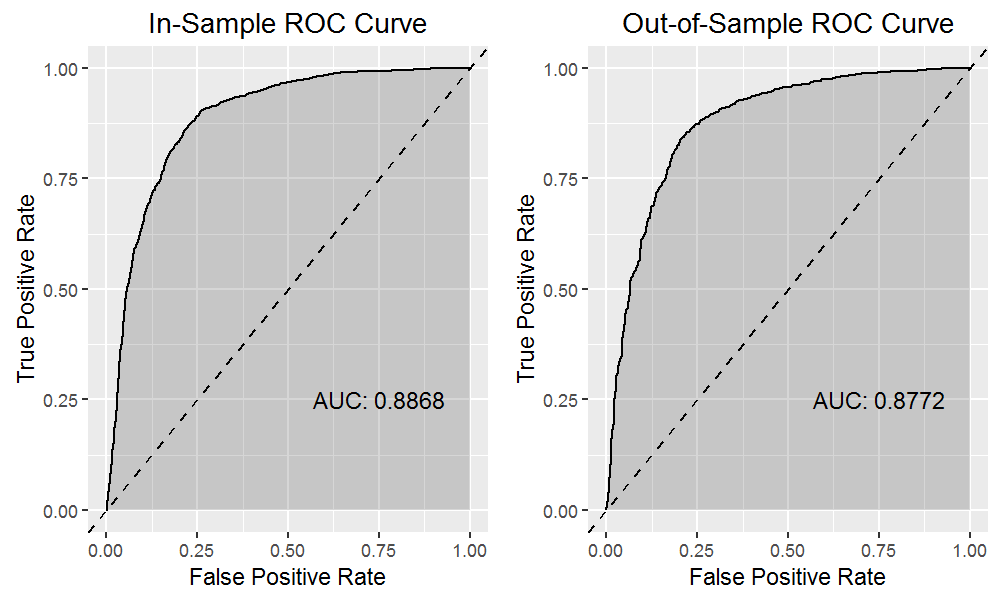
\includegraphics[height=2.60417in]{images/resp_nb_sample_roc.png}

\paragraph{Figure A.2 ROC Curve: Random
Forest}\label{figure-a.2-roc-curve-random-forest}

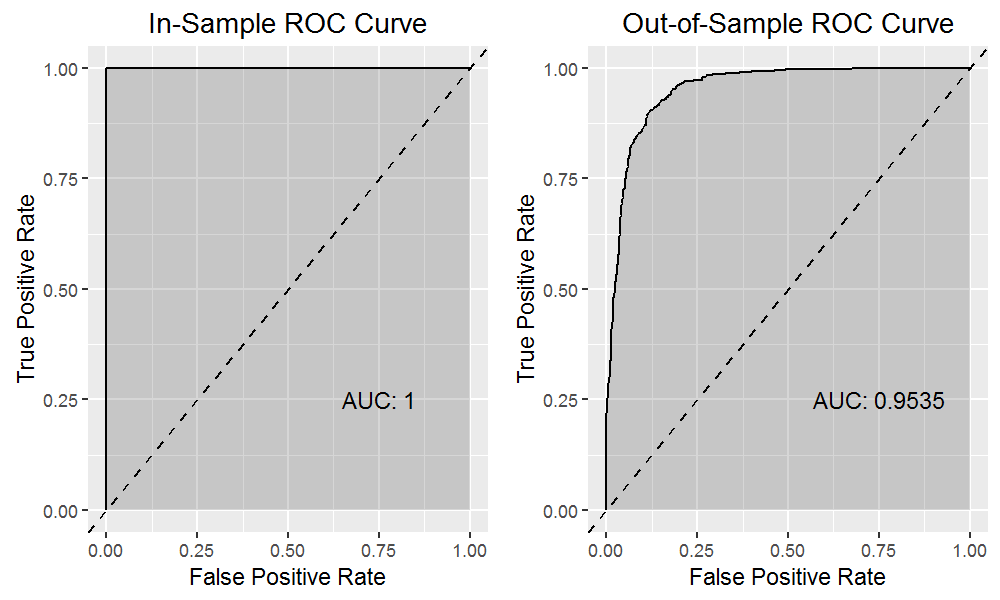
\includegraphics[height=2.60417in]{images/resp_rfc_sample_roc.png}

\paragraph{Figure A.3 ROC Curve: Lasso and Elastic-Net Regularized
Generalized Linear
Model}\label{figure-a.3-roc-curve-lasso-and-elastic-net-regularized-generalized-linear-model}

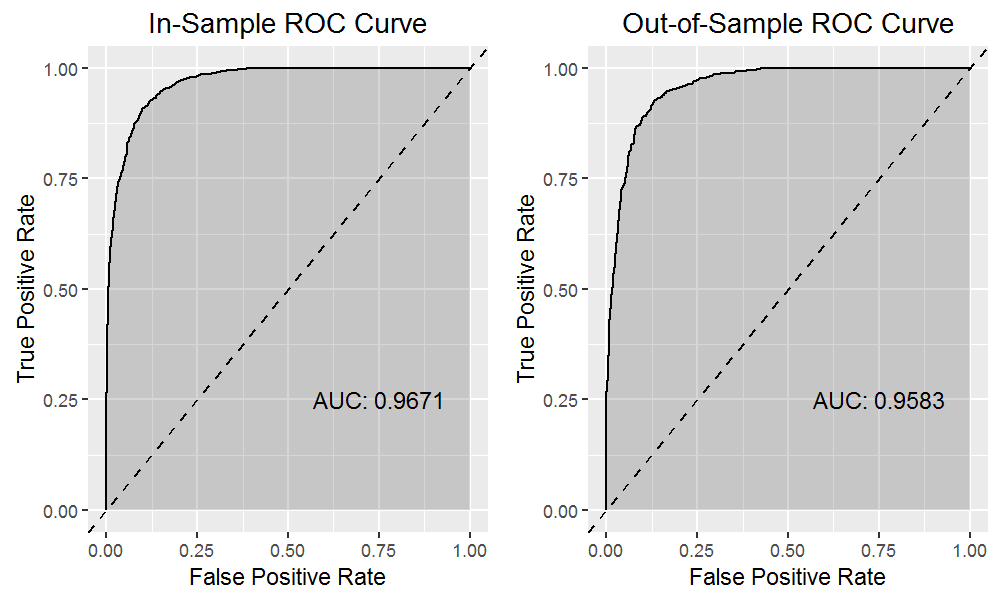
\includegraphics[height=2.60417in]{images/resp_glm_sample_roc.png}

\newpage

\paragraph{Figure A.4 ROC Curve: Logit
Boost}\label{figure-a.4-roc-curve-logit-boost}

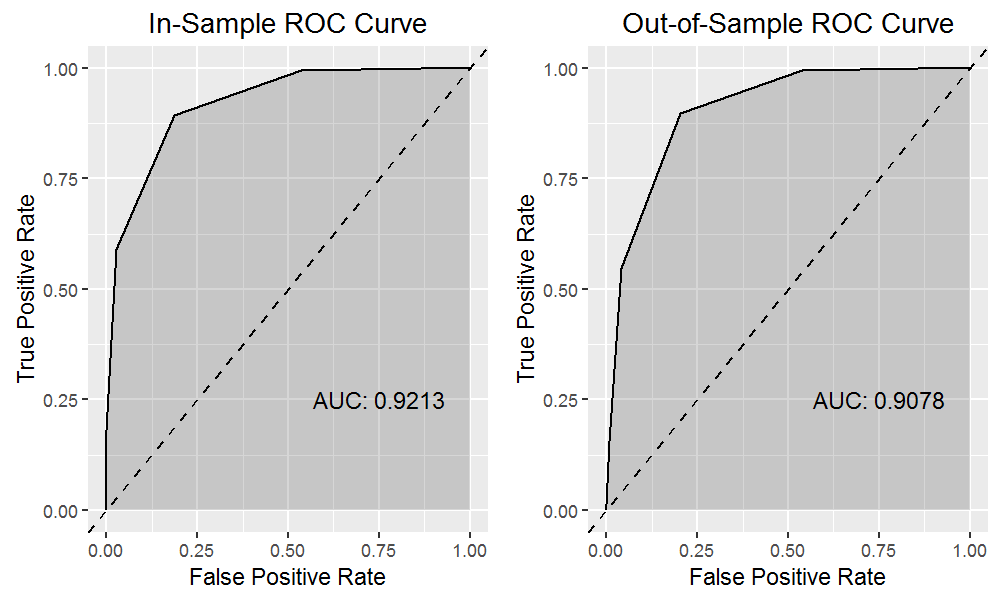
\includegraphics[height=2.60417in]{images/resp_lboost_sample_roc.png}

\paragraph{Figure A.5 ROC Curve: Linear Discriminant
Analysis}\label{figure-a.5-roc-curve-linear-discriminant-analysis}

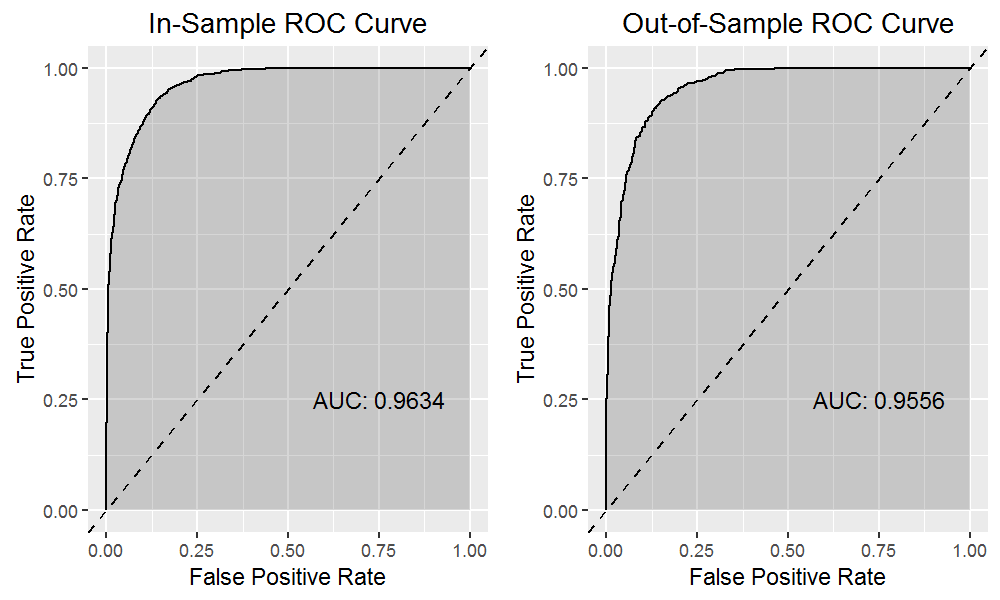
\includegraphics[height=2.60417in]{images/resp_lda_sample_roc.png}

\paragraph{Figure A.6 ROC Curve: k-Nearest
Neighbors}\label{figure-a.6-roc-curve-k-nearest-neighbors}

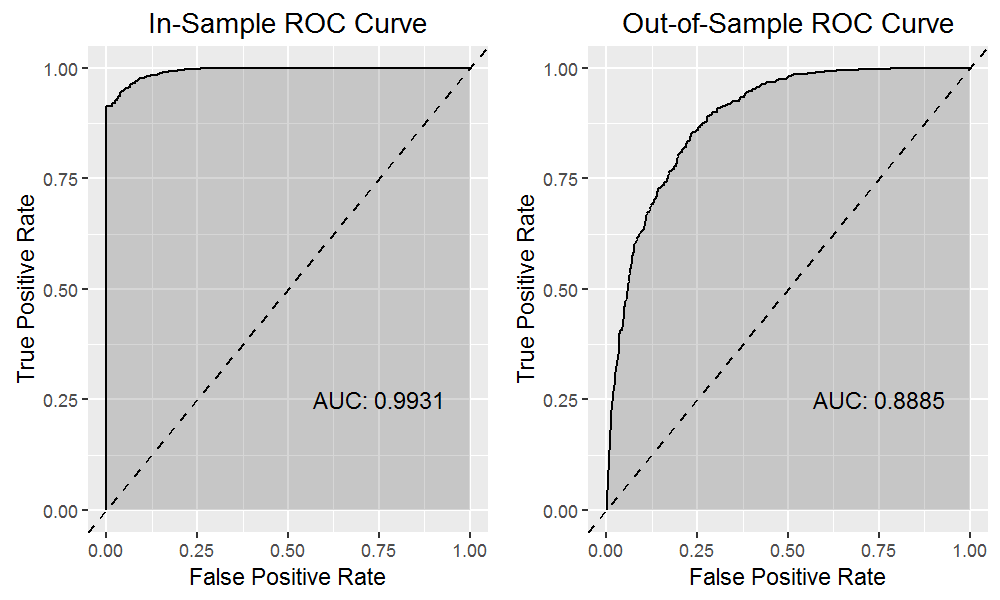
\includegraphics[height=2.60417in]{images/resp_knn_sample_roc.png}

\newpage

\paragraph{Figure A.7 Actuals vs.~Predictions: Multiple Linear
Regression}\label{figure-a.7-actuals-vs.predictions-multiple-linear-regression}

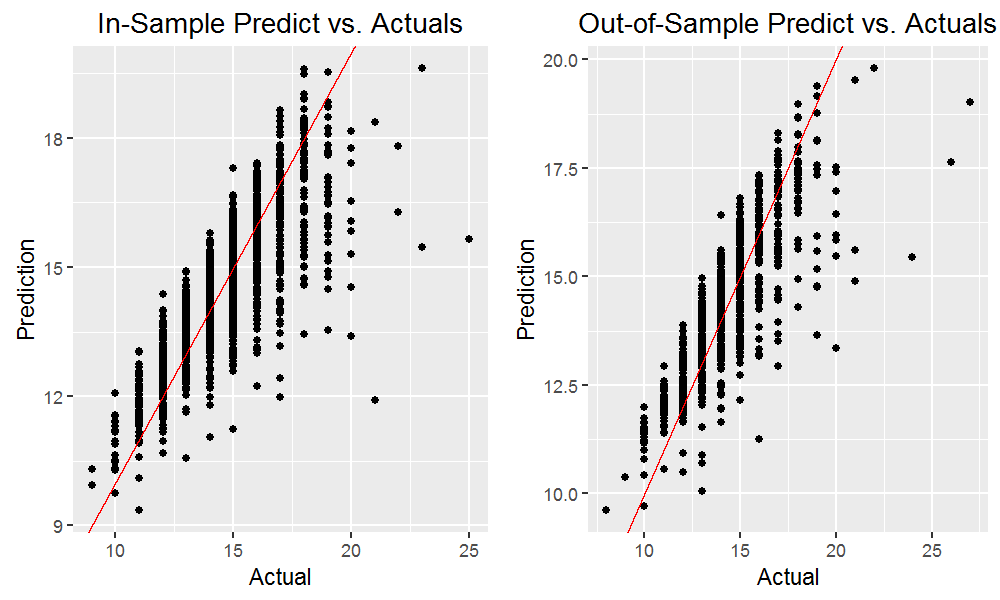
\includegraphics[height=2.60417in]{images/amt_lm_sample_pred.png}

\paragraph{Figure A.8 Actuals vs.~Predictions: Random
Forest}\label{figure-a.8-actuals-vs.predictions-random-forest}

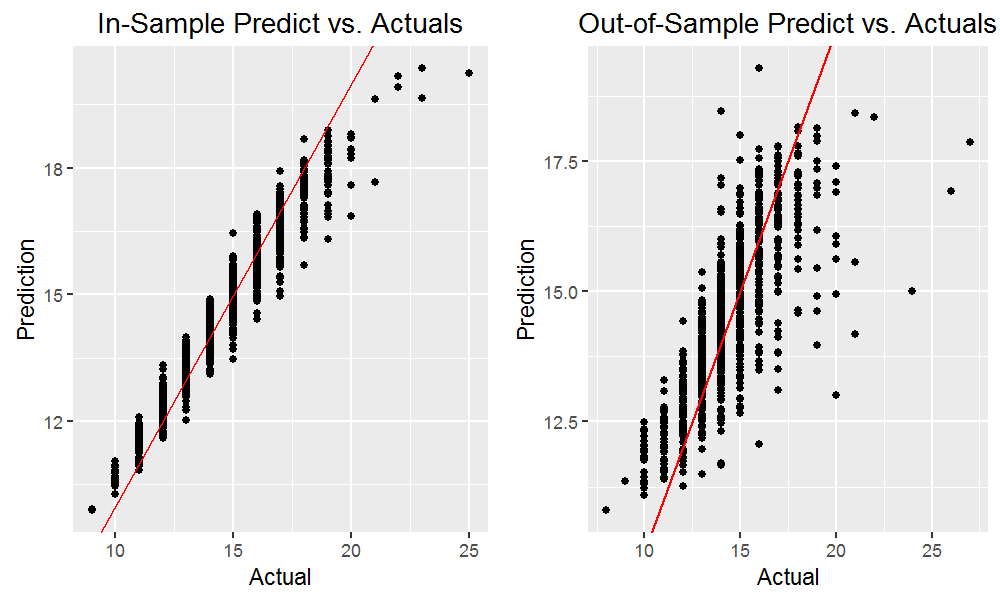
\includegraphics[height=2.60417in]{images/amt_rfr_sample_pred.png}

\paragraph{Figure A.9 Actuals vs.~Predictions: eXtreme Gradient
Boost}\label{figure-a.9-actuals-vs.predictions-extreme-gradient-boost}

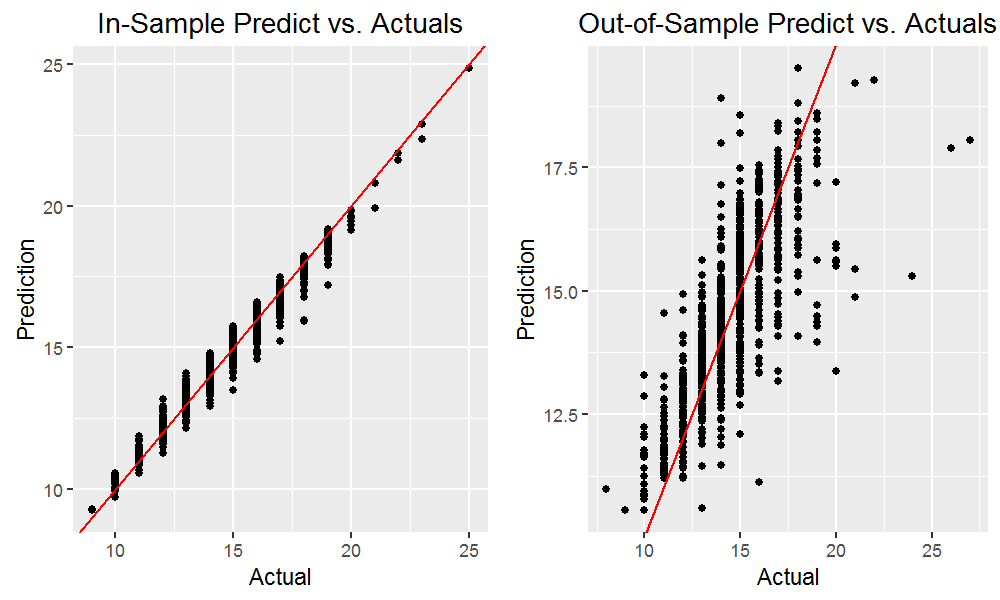
\includegraphics[height=2.60417in]{images/amt_xgb_sample_pred.png}

\newpage

\paragraph{Figure A.10 Actuals vs.~Predictions: Partial Least
Squares}\label{figure-a.10-actuals-vs.predictions-partial-least-squares}

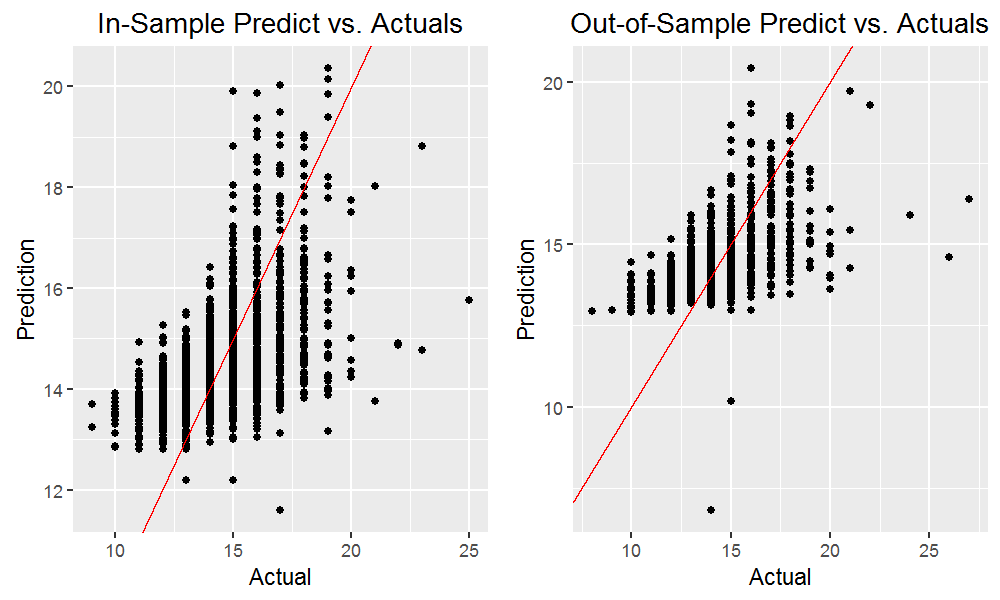
\includegraphics[height=2.60417in]{images/amt_pls_sample_pred.png}

\paragraph{Figure A.11 Actuals vs.~Predictions: Ridge
Regression}\label{figure-a.11-actuals-vs.predictions-ridge-regression}

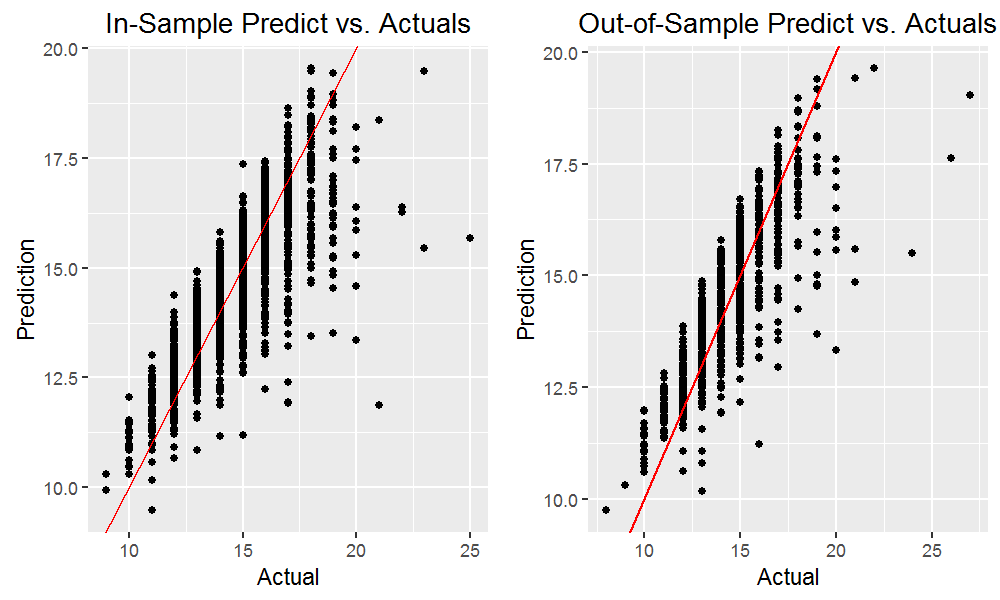
\includegraphics[height=2.60417in]{images/amt_rr_sample_pred.png}

\paragraph{Figure A.12 Actuals vs.~Predictions: Least Absolute Shrinkage
and Selection
Operator}\label{figure-a.12-actuals-vs.predictions-least-absolute-shrinkage-and-selection-operator}

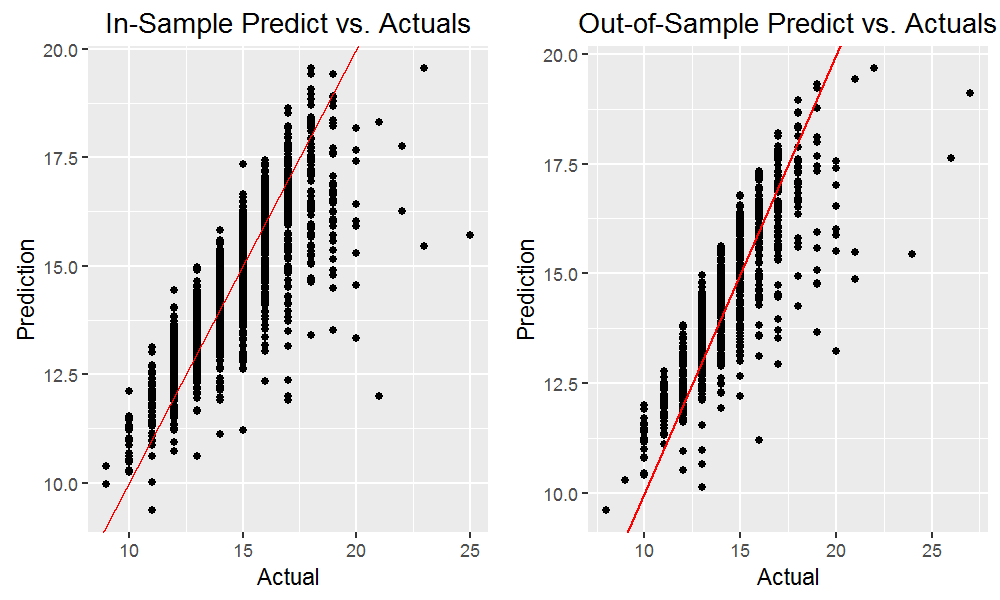
\includegraphics[height=2.60417in]{images/amt_lasso_sample_pred.png}


\end{document}
